% 2014 全国卷Ⅰ文科第 8 题：方格纸上的三视图。
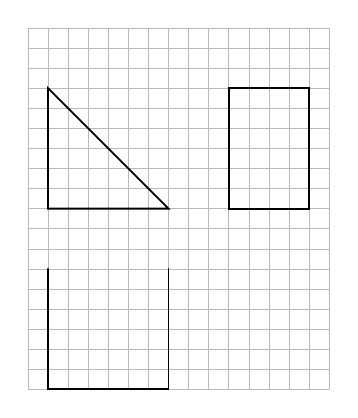
\begin{tikzpicture}[x=2.55mm,y=2.55mm,line cap=round]
  % 细灰色方格；粗实线是题面给出的三个投影。
  \draw[step=1,gray!55,line width=.18pt] (0,0) grid (15,18);
  \draw[line width=.65pt] (1,15)--(1,9)--(7,9)--cycle;
  \draw[line width=.65pt] (10,15)--(14,15)--(14,9)--(10,9)--cycle;
  \draw[line width=.65pt] (1,6)--(1,0)--(7,0)--(7,6);
\end{tikzpicture}
